% !TEX program = lualatex
\documentclass[aspectratio=169,professionalfonts]{beamer}
\usepackage{xcolor}
\usepackage{soul}
\sethlcolor{yellow}
\usepackage[table]{xcolor}  % Para colores en tablas
\usepackage{colortbl}       % Para sombreado por fila

%------------------------- Preamble (beamer) -------------------------%
%   Require LuaLaTeX + --shell-escape (for minted)                    %
%--------------------------------------------------------------------%
\usepackage[spanish]{babel}

% ---------- Fonts (modern look) ----------
\usepackage{fontspec}
\defaultfontfeatures{Ligatures=TeX, Scale=MatchLowercase}
\setmainfont{Inter}       % Sans‑serif body (install ttf–Inter)
\setsansfont{Inter}
\setmonofont{Fira Code}   % Nice mono for code

% ---------- Theme ----------
\usetheme[
  titleformat=smallcaps,
  numbering=fraction,
  progressbar=frametitle   % thin progress line under the title
]{metropolis}              % modern beamer theme
\metroset{block=fill}      % coloured blocks

% ---------- Colours ----------
\definecolor{clblue}{HTML}{005F9E}
\definecolor{clorange}{HTML}{FF9130}
\definecolor{clgrey}{HTML}{F4F4F4}

% ---------- minted ----------
\usepackage{minted}
\setminted{
  fontsize=\footnotesize,
  autogobble,
  breaklines,
  tabsize=2,
  style=monokai,
  linenos
}

% ---------- Custom boxes (tcolorbox) ----------
\usepackage{tcolorbox}
\tcbuselibrary{skins, breakable}
% Warning box
\newtcolorbox{warnbox}{
  colback=clorange!10,
  colframe=clorange!80!black,
  breakable,
  title={\faWarning\quad Advertencia},
  fonttitle=\bfseries,
  left=2mm, right=2mm, top=1mm, bottom=1mm
}
% Information box
\newtcolorbox{infobox}{
  colback=clblue!5,
  colframe=clblue!60!black,
  breakable,
  title={\faInfoCircle\quad Nota},
  fonttitle=\bfseries,
  left=2mm, right=2mm, top=1mm, bottom=1mm
}

% ---------- Icons ----------
\usepackage{fontawesome5}

% ---------- Misc tweaks ----------
\graphicspath{{figures/}}
\setlength{\parskip}{0.5em}
\addto\extrasspanish{\renewcommand{\contentsname}{Índice}}
%--------------------------------------------------------------------%




\title[ClústerLab • Día 5]{Introducción Slurm}
%\subtitle{Controlador y demonios de cómputo}
\author{ Catalina Victoria Ruiz Equipo docente ClústerLab}
\date{13 de agosto de 2025}

\begin{document}

%------------------------------ portada ----------------------------
\begin{frame}[plain]
  \titlepage
\end{frame}

%------------------------------ objetivos --------------------------
\begin{frame}[fragile]
\frametitle{\textbf{Objetivos de la sesión}}
  \begin{itemize}
\item Conociendo Infraestructura NLHPC 
         \vspace{0.5em} 
\item Acceso Cluster NLHPC mediante \texttt{ssh}
         \vspace{0.5em} 
\item Copiar archivos 
\vspace{0.5em} 
\item \textbf{SLURM}
\vspace{0.5em} 
\item Acceso módulos de software 
\vspace{0.5em} 
\item Monitoreo tareas y asignación de recursos
\vspace{0.5em} 
\item Let's play and have fun  !! 
\end{itemize}
\end{frame}



\begin{frame}[fragile]
\frametitle{\textbf{Infraestructura NLHPC: Leftaru y Guacolda}}
    \centering
    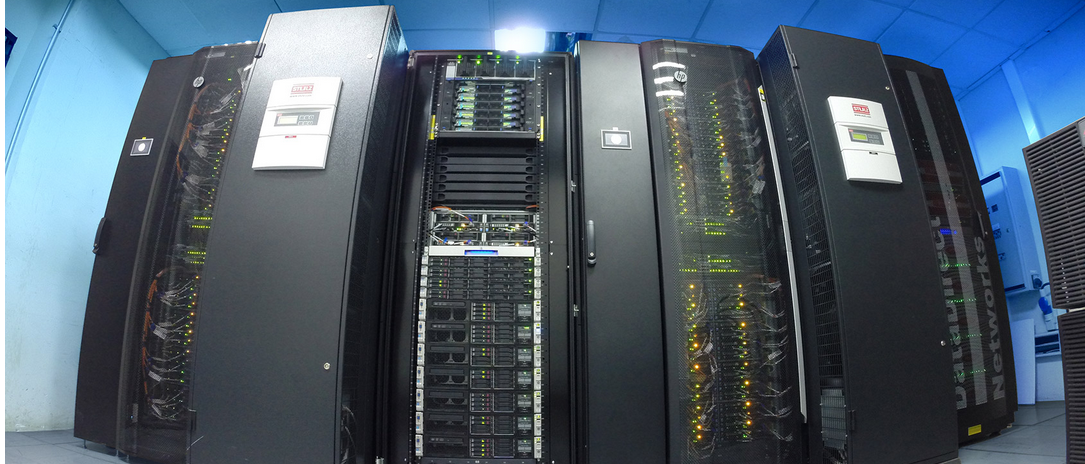
\includegraphics[scale=0.3]{FIGURES/NLHPC.png}
    
    \vspace{0.5em}
    {\color{blue} \scriptsize \texttt{https://www.nlhpc.cl/infraestructura/}}
\end{frame}


\begin{frame}[fragile]
\frametitle{\textbf{Infraestructura: Leftraru (AMD)}}
    \begin{center}
            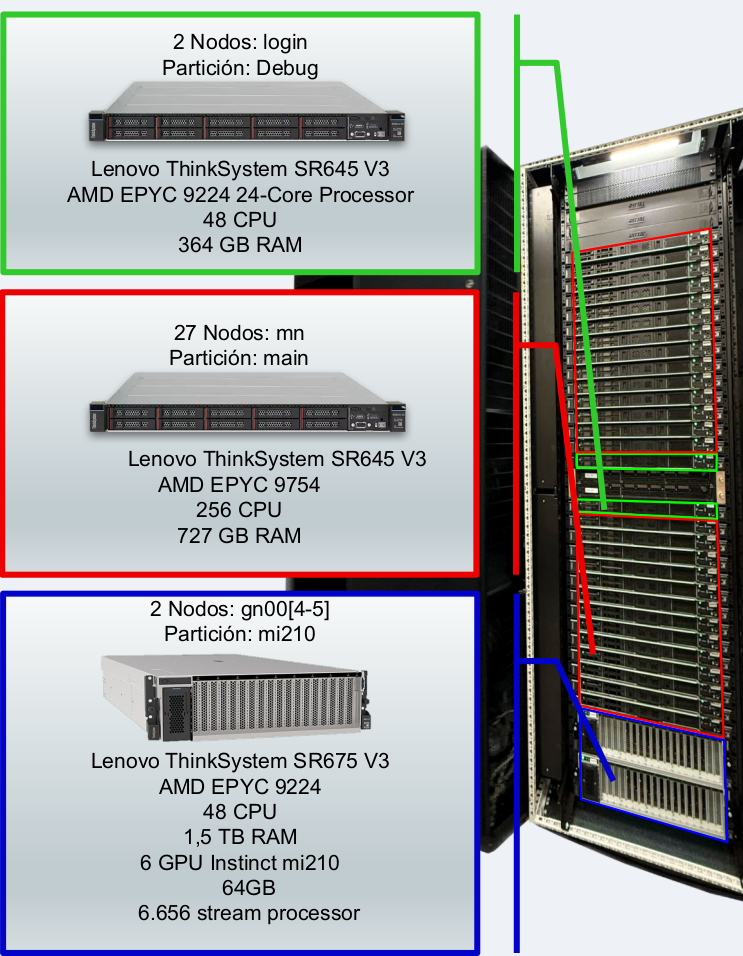
\includegraphics[scale=0.2]{FIGURES/leftraru.png}
    \end{center}    
\end{frame}

\begin{frame}{\textbf{Infraestructura: Guacolda (INTEL)}}
    \begin{center}
            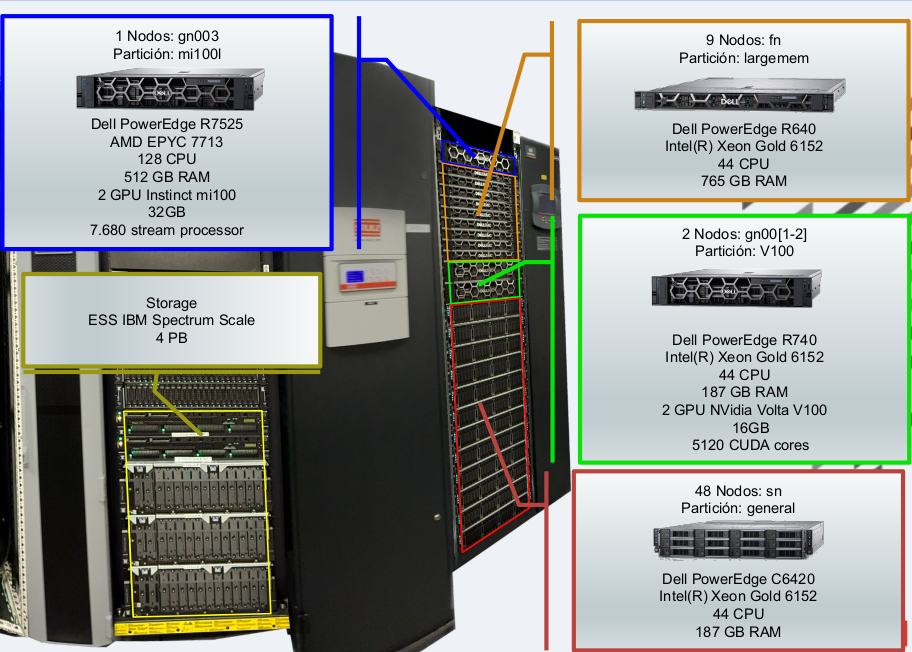
\includegraphics[scale=0.3]{FIGURES/guacolda.png}

    \end{center}
    
\end{frame}


\begin{frame}[fragile]
\frametitle{\textbf{Infraestructura General}}
\begin{itemize}
    \item General : 9828 CPU
        \vspace{0.5em} % espacio vertical después del ítem
    \item Potencia : 479 TFlops
        \vspace{0.5em} % espacio vertical después del ítem
    \item Almacenamiento: 4 PB IBM Spectrum Scale
        \vspace{0.5em} 
    \item Comunicación: Red LAN infiniband NDR 100Gbps
\end{itemize}
    
\end{frame}




\begin{frame}[fragile]
\frametitle{\textbf{Acceso Cluster}}

Para acceder al Cluster: 
\begin{itemize}
    \item Cuenta + contraseña (Ustedes ya la tienen. \hl{no cambiar contraseña!})
    
    \item Utilizar comando: 
     \begin{minted}{bash}
$ ssh -p 4603 fantastic$_$user@leftraru.nlhpc.cl
  \end{minted}
    \item Primera conexión: Confirmar con 
    \begin{minted}{bash}
    $ yes 
    \end{minted} 
    \item  OJO! no necesariamente tiene que entrar por terminal (LINUX). Otras opciones (Windows): 
        \begin{itemize}
            \item PowerShell
            \item Putty
        \end{itemize}
    \end{itemize}
    \centering
    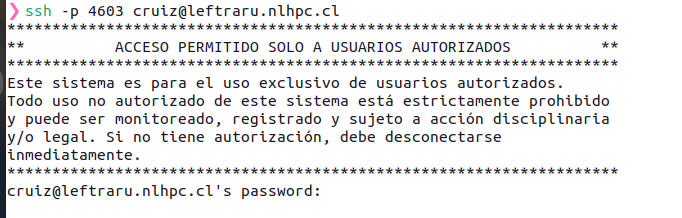
\includegraphics[scale=0.3]{FIGURES/ssh_2.png}
     \vspace{0.5em}
\end{frame}

\begin{frame}[fragile]
\frametitle{\textbf{¡Entramos!}}
\begin{itemize}
    \item Una vez entren al Cluster verán algo como esto: 
\end{itemize}
\centering

\includegraphics[scale=0.2]{FIGURES/log_in_1.png}
 \vspace{0.5em}
   %  {\scriptsize \texttt{Ingreso exitoso}}
\end{frame}


\begin{frame}[fragile]
\frametitle{\textbf{Primeros Pasos en NLHPC}}
\begin{itemize}
    \item ¿Qué significa leftraru1 o leftraru2? 
            \vspace{0.5em} 

    \item Partición \texttt{debug}: 2 nodos login 
            \vspace{0.5em} 

    \item Tiempo máximo en \texttt{debug} 30 minutos 
            \vspace{0.5em} 

    \item ¿Cómo llego a las otras partición? $\rightarrow$ \textbf{SLURM}. Take it easy, we will go for it
\end{itemize}
    
\end{frame}


\begin{frame}[fragile]
\frametitle{\textbf{Acceso Llaves}}
\begin{itemize}
    \item Acceso sin pedir contraseña
            \vspace{0.5em} 

    \item Resguardar nuestro acceso 
            \vspace{0.5em} 

    \item Evita ingreso incorrecto de contraseñas
    
\end{itemize}
    
\end{frame}

\begin{frame} [fragile]
\frametitle{\textbf{Crear llave SSH}}
\begin{itemize}
    \item Crear llave:
    \end{itemize}
    \begin{minted}{bash}
        $ ssh-keygen -t ed25519} 
        $ 3 enter
    \end{minted}
    
    \begin{itemize}
        \item Copiar llave:
    \end{itemize}

\begin{minted}{bash}
$ ssh-copy-id -p 4603 fantastic$_$user@leftraru.nlhpc.cl
    \end{minted}
\begin{itemize}
    \item Solicita Clave acceso
    \item Mensaje de confirmación
\item Ingresa al Cluster 
\item Probemos el primer comando : \texttt{usoDisco} o \texttt{df}
\item Listemos nuestro home: \texttt{ls}

    \end{itemize}
\end{frame}

\begin{frame}[fragile]
\frametitle{\textbf{Traspaso Archivos desde/al Cluster}}
Sintáxis Básica: \\
\begin{minted}{bash}
    $   {scp  [opciones] origen destino} \\
\end{minted}
\vspace{0.5em}
Opciones comunes:
    \begin{itemize}
        \item -r: Copia recursiva
        \vspace{0.5em}
        \item -P: Especifica el puerto SSH
        \vspace{0.5em}
        \item -v: Modo \textit{verbose}
    \end{itemize}
\end{frame}


\begin{frame}[fragile]
\frametitle{\textbf{Hands on!}}
\begin{itemize}
    \item  Descarga el archivo para copiarlo en tu \textit{home} de leftraru
    \item Verifica tu ruta de origen con \texttt{pwd} (Ya conoces la de destino) 
    \item     Copia el archivo de interés a tu \textit{home} de leftraru.
\end{itemize}
Ejemplo: \\
\begin{minted}{bash}
    $ scp -P 4603 /home/catalina/Descargas/archivo-descargado.dat cruiz@leftraru.nlhpc.cl: \hl{~}} \\
    $ scp -P 4603 /home/catalina/Descargas/archivo-descargado.dat cruiz@leftraru.nlhpc.cl:\hl{/home/cruiz}
\end{minted}
\end{frame}



\begin{frame}[fragile]
\frametitle{\textbf{¿Y si no quiero dejarlo en el \textit{home}?}}
\begin{itemize}
    \item Crea tu carpeta/directorio:
    \end{itemize}
    \begin{minted}{bash}
        $  \hl{mkdir nombre-carpeta}
    \end{minted}
   \begin{itemize}
       \item  \item Entra a tu carpeta/directorio:
   \end{itemize}
   \begin{minted}{bash}
       $ \hl{cd nombre-carpeta}
   \end{minted}
    ¡Vamos de nuevo!
   \begin{minted}{bash}
       $ scp -P 4603 /home/catalina/Descargas/archivo-descargado.dat cruiz@leftraru.nlhpc.cl:\hl{~/CL2025}
   \end{minted}
   \begin{itemize}
       \item Lista tu carpeta/directorio: ls 
   \end{itemize}
       
\end{frame}

\begin{frame}[fragile]
\frametitle{\textbf{Otras formas de traspasar archivos}}
\begin{itemize}
    \item rsync $\rightarrow$ \texttt{rsync [opciones] origen destino}
    \vspace{0.5em} 
    \item Filezilla usando sftp $\rightarrow$ {\color{blue} \scriptsize \texttt{https://filezilla-project.org/}}
    \end{itemize}
    
\end{frame}




\begin{frame}[fragile]
\frametitle{\textbf{Simple Linux Utility for Resource Management}}
\begin{itemize}
    \item  Permite acceder al poder de cómputo del Clúster
    \vspace{0.5em} 
    \item Entrega información del estado de los nodos y tareas (\textit{jobs})
    \vspace{0.5em} 
    \item Permite ejecución de tareas de manera interactiva 
    \vspace{0.5em} 
    \item Gestión de tareas en cola de trabajo 
    \vspace{0.5em} 
    \item Gestiona recursos computacionales 
    \vspace{0.5em} 
    \item Permite, actualmente, ejecutar tareas hasta por 30 días
    
\end{itemize}
    
\end{frame}

\begin{frame}{\textbf{SLURM-Gestor de Recursos}}
A través de SLURM podemos lanzar \textit{jobs} hacia las distintas particiones de NLHPC: debug, main, general, largemem, v100, mi100 y mi210. Ejecución máxima : 30 días. \\\\ 
\vspace{0.5em}
¿Qué ocurre con debug ?
    
\end{frame}


\begin{frame}[fragile]
\frametitle{\textbf{SLURM: Comandos básicos}}
\begin{itemize}
    \item \texttt{sinfo} : 
    \begin{itemize}
        \item Nombre partición
        \item Disponibilidad
        \item Límite tiempo por partición
        \item Número y listado de nodos
        \item Estados:
        \begin{itemize}
            \item Disponible (\texttt{idle})
            \item Ocupados por completo (\texttt{alloc})
            \item Ocupados con recursos disponibles (\texttt{mix})
            \item Reservados (\texttt{resv})
            \item Vaciado/vaciando (\texttt{drain/drng})
        \end{itemize}
        
    \end{itemize}
\end{itemize}
\end{frame}

\begin{frame}[fragile]
\frametitle{\textbf{Visualizando sinfo}}
  \centering
    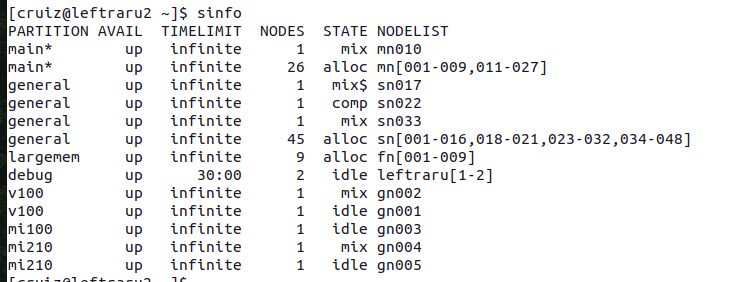
\includegraphics[scale=0.3]{FIGURES/sinfo.png}   
    \begin{itemize}
        \item Pero nosotros tenemos una partición especial para esta escuela:  \\ \hl{labs} 
    \end{itemize}
    \begin{minted}{bash}
        $ sinfo -a 
    \end{minted}
\end{frame}
\begin{frame}[fragile]
\frametitle{\textbf{Visualizando sinfo-a}}
\centering
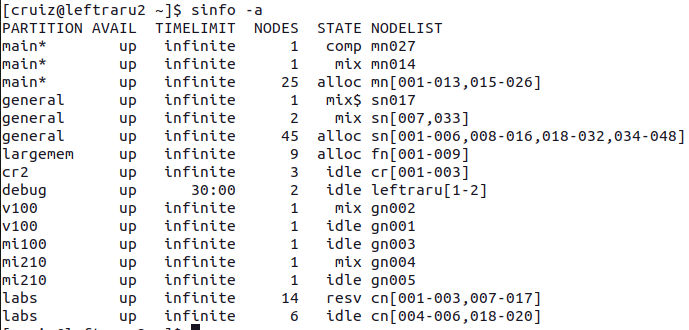
\includegraphics[scale=0.3]{FIGURES/sinfo-a.png}
\end{frame}


\begin{frame}[fragile]
\frametitle{\textbf{SLURM: srun}}
\textbf{srun} para ejecutar jobs en modo interactivo 
\begin{itemize}
    \item Ejecuta un programa o script en los nodos de cómputo
    \item Recibe parámetros o utiliza valores por defecto
    \item Asigna un JobID  a nuestro job
    \item No libera la terminal, ie, si cierra sesión la aplicación fallará. 
\end{itemize}
    Sintáxis: 
\begin{minted}{bash}
    $ {srun} [parámetros] \textbf{ejecutable} [argumentos]
\end{minted}

   
    Ejemplos: 

\begin{minted}{bash}
    $ srun hostname
    $ srun} - p general hostname
    $ srun} -p main -n 2 --ntask-per-node=1 hostname
\end{minted}
 
\end{frame}


\begin{frame}[fragile]
\frametitle{\textbf{Primeros scripts en SLURM}}
\begin{itemize}
    \item Empezamos utilizando un editor de texto : vim (vi), nano. 
    \item Le colocamos un nombre al script (as you wish) con terminación .sh (EJ: job1.sh, first.sh, 1.sh, etc)
    \item Escribimos:
\end{itemize}

\begin{minted}{bash}
    $ \#\!/usr/bin/bash
    $ echo "Este es nuestro primer script del curso SLURM "
    $ echo
    $ echo "Este script se ha ejecutado en el nodo \$\textbackslash(hostname)"
    $ echo 
\end{minted}


    \begin{itemize}
        \item \hl{Ojo con la primera línea del script}
        \item Corremos con \hl{sbatch job1.sh}
        \item Revisamos la salida 
    \end{itemize}
    \end{frame}

\begin{frame}[fragile]
{\textbf{Sigamos con nuestro primer script}}
\begin{itemize}
    \item Prueba con \textbf{srun}\vspace{0.5em}
    \vspace{0.5em}
    \item Ingresa parámetros a \textbf{srun}:
    \vspace{0.5em}
   \end{itemize} 



  \begin{minted}{bash}
  $ srun -p general ejercicio1.sh
  $ srun -n 2 --ntaks-per-node=1 ejercicio1.sh
  $ srun -p general -n 3 --ntasks-per-node=1 ejercicio1.sh
  \end{minted} 
  \vspace{0.5em}
    \begin{itemize}
        \item ¿Qué diferencias hay?
    \end{itemize}
    \end{frame}

\begin{frame}[fragile]
\frametitle{\textbf{SLURM: Asignación de recursos}}
\begin{itemize}
    \item Se pueden utilizar con \textbf{srun} o con \textbf{sbatch}
    \vspace{0.5em}
    \item Permite asignar recursos de cómputo:
    \vspace{0.5em}
    \begin{itemize}
        \item Particiones
        \item Número de procesos
        \item CPU por procesos
        \item Memoria RAM
    \end{itemize}
    \item Define los archivos de salida y error
    \vspace{0.5em}
    \item Permite comunicación con el usuario
\end{itemize}
    
\end{frame}


\begin{frame}[fragile]
\frametitle{\textbf{Parámetros comunes en SLURM}}
\scriptsize
\rowcolors{2}{gray!10}{white}
\begin{tabular}{|p{2.5cm}|p{5.5cm}|p{4.5cm}|}
\hline
\rowcolor{blue!20}
\textbf{Parámetro} & \textbf{Ejemplo de uso} & \textbf{Acción} \\
\hline
-J & \texttt{-J \_nombre\_tarea} & Asigna un nombre a nuestra tarea \\
-p & \texttt{-p main} & Indica la partición a utilizar \\
-n & \texttt{-n 4} & Número de procesos \\
-c & \texttt{-c 5} & CPU por proceso \\
--mem-per-cpu & \texttt{--mem-per-cpu=1000} & RAM por CPU \\
--ntasks-per-node & \texttt{--ntasks-per-node=4} & Procesos por nodo \\
-o & \texttt{-o archivo\_salida\_\%\j.out} & Registro/Log de salida \\
-e & \texttt{-e archivo\_salida\_\%\j.err} & Registro/Log de errores \\
--mail-user & \texttt{--mail-user=fantasticuser@gmail.com} & Correo para envío de información \\
--mail-type & \texttt{--mail-type=ALL} & Información a enviar \\
\hline
\end{tabular}
\end{frame}


\begin{frame}[fragile]
\frametitle{\textbf{¿Y los parámetros por defecto?}}
\begin{itemize}
    \item Partición: main  (-p main)
    \vspace{0.5em}
    \item  Número procesos: 1  (-n 1)
    \vspace{0.5em}
    \item Número CPU: 1 (-c 1)
    \vspace{0.5em}
    \item  Memoria: 1000M (--mem-per-cpu=1000)
    \vspace{0.5em}
    \item Tareas por proceso: 1 (--ntasks-per-node=1)
\end{itemize}
    \hl{OJO} Los parámetros de SLURM se utilizan tanto en modo interactivo (\textbf{srun}) como en scripts de jobs (\textbf{sbatch})
\end{frame}
\begin{frame} [fragile]
\frametitle{\textbf{SLURM: Uso scripts}}
    \begin{itemize}
        \item Permite asignar recursos de cómputo 
         \vspace{0.5em} 
        \item Los job se envían a una cola de trabajo con un JobID \textbf{único} \\ $\rightarrow$ \hl{squeue y/o squeue -a}
         \vspace{0.5em} 
        \item  Monitorear jobs
         \vspace{0.5em} 
        \item No requiere sesión activa, al contrario con \textbf{srun}
    \end{itemize}
\end{frame}


\begin{frame}[fragile]
\frametitle{\textbf{SLURM:Enviar tareas}}
    \texttt{\#\!/usr/bin/bash} \\
\texttt{\#SBATCH -J mi\_tarea} \\
\texttt{\#SBATCH -p main} \\
\texttt{\#SBATCH -n 1} \\
\texttt{\#SBATCH -c 1} \\
\texttt{\#SBATCH --mem-per-cpu=1000} \\
\texttt{\#SBATCH -o archivo\_salida\_\%j.out} \\
\texttt{\#SBATCH --mail-user=fantasticuser@gmail.com} \\
\texttt{\#SBATCH --mail-type=ALL} \\
\\
\texttt{echo ``inicio de mi programa''} \\
\texttt{mi\_programa parametros} \\
\texttt{echo ``fin de mi programa''} \\
\end{frame}
    
\begin{frame}{\textbf{Comandos SLURM}}
    \begin{itemize}
        \item \textbf{squeue} y/o \textbf{squeue -a}
         \vspace{0.5em} 
        \item \textbf{scancel JobID}
         \vspace{0.5em} 
        \item \textbf{scontrol -dd show job JobID}
         \vspace{0.5em} 
        \item \textbf{sacct -X}
        
    \end{itemize}
\end{frame}


\begin{frame}[fragile]{\textbf{Sigamos...}}


\begin{minted}{bash}
$ \#\!/bin/bash 
$ \#SBATCH -J ejercicio2 
$ \#SBATCH -p labs 
$ \#SBATCH -t 0:15:00 
$ \#SBATCH -o logs/ejercicio2\_\%j.out 
$ \# ----------------Modulos---------------------------- 
$ ml intel/2022.00
$ ml Python/3.9.5 
$ \# ----------------Comando-------------------------- 
$ python simular\_consumo\_cpu.py 1
\end{minted}



\begin{itemize}
    \item ¿Qué parámetros tiene? ¿Falta alguno?
         \vspace{0.5em} 
    \item Asigna 1 proceso y 1 cpu
         \vspace{0.5em} 
    \item Lanza el job a la cola de trabajo
         \vspace{0.5em} 
    \item Monitorea tu job (en detalle)
         \vspace{0.5em} 
    \item Puedes cancelar 
\end{itemize}
    
\end{frame}

\begin{frame}[fragile]
\frametitle{\textbf{General Questions}}
\begin{itemize}
    \item ¿Diferencia entre un nodo de cómputo y partición?
     \vspace{0.5em} 
    \item ¿Cómo puedo saber el espacio que tengo disponible?
     \vspace{0.5em} 
    \item ¿Cúales son las particiones disponibles?
     \vspace{0.5em} 
    \item ¿Diferencia entre srun y sbatch?
     \vspace{0.5em} 
    \item ¿Cómo monitoreo mis jobs?
     \vspace{0.5em} 
    \item ¿Cómo cancelo mi job?
\end{itemize}
    
\end{frame}

\begin{frame}[fragile]

\vspace{0.5em} 
\textbf{Let's take a break...}
    
\end{frame}


\begin{frame}[fragile]
\frametitle{\textbf{LMOD: Accediendo a software mediante módulos}}
  Sintáxis: \\ 
  ml [comando]  [software[/version]] \\ 
  Comandos: \\ 

  \begin{minted}{bash}
        $ purge: Elimina módulos cargados  
   $ avail: Lista módulos disponibles  
     $ spider: Busca módulos disponibles según palabra clave.
      $ software: Carga el módulo de software disponible. 
       $ show software/version: Muestra detalles del módulo.
  \end{minted}

\end{frame}

\begin{frame}{\textbf{LMOD}}
    \texttt{ml} para ver módulos cargados \\ 
    \texttt{ml spider Python} para buscar módulos\\ 
\centering
    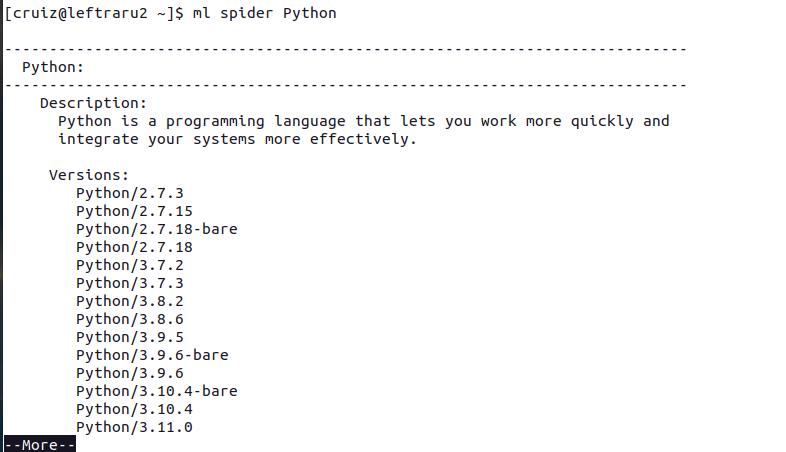
\includegraphics[scale=0.25]{FIGURES/ml_spider_python.png} \\
\end{frame} 

\begin{frame}[fragile]
\frametitle{\textbf{LMOD}}
\begin{minted}{bash}
$ ml spider Python/3.8.2
$ ml spider wrf
$ ml spider WRF
    
\end{minted}



\end{frame}

\begin{frame}{fragile}
\frametitle{\textbf{WorkTime!}}
Descarge y copie el archivo ejercicio.intel.job, para cumplir lo siguiente:
\begin{itemize}
    \item Utiliza partición labs 
         \vspace{0.5em} 
    \item Reserva 1 proceso y 2 cpus
         \vspace{0.5em} 
    \item Reserva 2000 MB de memoria RAM total   
    \vspace{0.5em} 
     \item Busca la versión de R compiladas
          \vspace{0.5em} 
   \item Carga la versión 4.4.0 
        \vspace{0.5em} 
    \item Ejecute el script 
         \vspace{0.5em} 
    \item Busque la versión R 4.4.0 correspondiente a procesadores AMD 
    
\end{itemize}
    
\end{frame}


\begin{frame}[fragile]
\frametitle{\textbf{Keep Working}}
Descargue y copie el archivo job4.sh
    \begin{itemize}
        \item Asigne 5 procesos con 1 CPU cada uno 
         \vspace{0.5em} 
        \item Asigne sus archivos de error y salida
         \vspace{0.5em} 
        \item Haga correr su job 
         \vspace{0.5em} 
        \item Monitoree entrando al nodo de cómputo: 
        \end{itemize}
        \begin{minted}{bash}
            $ ssh nodo00
            $ htop
        \end{minted}
      \begin{itemize}
          \item¿Cómo lo arreglo?
      \end{itemize}
  
\end{frame}

\begin{frame}[fragile]
\frametitle{\textbf{Asignación Memoria}}
    Hay jobs que exigen mucha memoria RAM, y según la partición es la capacidad que tendrá(general o largemem). Recordemos que el \textit{default} es 1000M
    \begin{itemize}
        \item Exceeded job memory limit 
         \vspace{0.5em} 
        \item Out of Memory 
         \vspace{0.5em} 
        \item OOM Error 
    \end{itemize}
\end{frame}


\begin{frame}[fragile]
\frametitle{\textbf{Last Exercise!}}
Vamos con el job5.sh (último de hoy)
\begin{itemize}
    \item Generando el error
     \vspace{0.5em} 
    \item ¿Cómo lo arreglo?. Veamos los logs de errores. 
\end{itemize}
    
\end{frame}

\begin{frame}[fragile]
\frametitle{\textbf{Finalizando...}}

\begin{itemize}
    \item dashboard.nlhpc.cl
     \vspace{0.5em} 
    \item wiki.nlhpc.cl
     \vspace{0.5em} 
    \item soporte NLHPC 
     \vspace{0.5em} 
    \item Generador de \texttt{scripts}
     \vspace{0.5em} 
    \item \textbf{Ustedes podrían tener acceso personal NLHPC }
     \vspace{0.5em} 
    \item Next Step? Paralelismo
\end{itemize}
\end{frame}
    \begin{frame}
 \vspace{0.5em} 
    \textbf{¡MUCHAS GRACIAS !}
        
    \end{frame}
\end{document}